\documentclass[14pt,a4paper,titlepage]{extarticle}
\usepackage[utf8]{inputenc}
\usepackage[english,ukrainian]{babel}
\linespread{1} %полуторный межстрочный интервал
\usepackage[pdftex,left=2cm,right=2cm,top=2cm,bottom=2cm]{geometry} %поля
\pagestyle{myheadings} %номер страниц
\usepackage{indentfirst} %чтобы абзац после названия раздела был с красной строки
\parindent=1.25cm %красная строка 1,25см
\righthyphenmin=2 %чтобы 2 последние буквы слова переносились тоже
\sloppy %выривнивание по ширине
\usepackage{amssymb}
\usepackage{amsmath}
\usepackage{verbatim}

\makeatletter 
\renewcommand{\@biblabel}[1]{#1.}
\usepackage{misccorr} %для точки после номера раздела

\usepackage[table,xcdraw]{xcolor}

\newcommand{\RomanNumeralCaps}[1]
    {\MakeUppercase{\romannumeral #1}}

\usepackage{graphicx}
\graphicspath{{pictures/}}
\DeclareGraphicsExtensions{.png,.jpg}

\begin{document}
      \begin{titlepage}
      %\thispagestyle{empty}
         \begin{center}
ДНІПРОВСЬКИЙ НАЦІОНАЛЬНИЙ УНІВЕРСИТЕТ ІМ. О. ГОНЧАРА\\
ФАКУЛЬТЕТ ПРИКЛАДНОЇ МАТЕМАТИКИ\\
КАФЕДРА ОБЧИСЛЮВАЛЬНОЇ МАТЕМАТИКИ ТА МЕТЕМАТИЧНОЇ
КІБЕРНЕТИКИ\\
            \vspace{6cm}
            \bf Лабораторна робота №3\\
            \bf <<МЕТОДИ РОЗВ’ЯЗУВАННЯ НЕЛІНІЙНОГО РІВНЯННЯ>>\\
            \bf з курсу <<Методи обчислень>>\\
            \bf Варіант №2
        \end{center}
        \vspace{5cm}
        \begin{flushright}
Виконав:\\
студент групи ПА-18-1(2)\\
Лєшанов Андрій
        \end{flushright}
        \begin{center}
        \vspace{5.5cm}
        Дніпро, 2020
        \end{center}
   \end{titlepage}
\setcounter{page}{2}
\newpage
{\centering\tableofcontents}
\newpage
{\centering \section*{Постановка задачі}}
\addcontentsline{toc}{section}{Постановка задачі}

Розглянемо рівняння
\begin{equation}
f(x)=0,\text{ де } f(x)\in C[a,\, b].
\end{equation}

Число $\xi$, що перетворює рівняння (1) у тотожність, будемо називати коренем цього рівняння, або нулем функції $f(x)$. Розв'язати рівняння - означає знайти всі його корені. Корені рівняння можуть бути дійсними, комплексними, кратними, ізольованими (простими).

Лише у виняткових випадках розв'язок рівняння можна побудувати у вигляді формули. Крім того, у деяких випадках рівняння (1) може мати коефіцієнти, які відомі лише наближено, тоді задача про точне визначення коренів такого рівняння втрачає сенс.

Наближений пошук ізольованих дійсних коренів складається з двох етапів: відокремлення коренів і уточнення.

Відокремити дійсний корінь - означає знайти інтервал (за можливістю малий), який містить лише один корінь рівняння.

Уточнити корінь - означає довести його наближене значення до потрібної точності.
\newpage
{\centering \section{Основні теоретичні відомості}}
{\centering \subsection{Методи відокремлення дійсних коренів}}

При відокремленні дійсних коренів аналітичним методом слід опиратися на першу теорему Больцано-Коші.

{\bf Теорема.} Якщо визначена і неперервна на відрізку $[a,\, b]$ функція $f(x)$ приймає на кінцях цього відрізку значення різних знаків, тобто $f(a)\cdot f(b)<0$, то цей відрізок містить хоча б 1 дійсний корінь рівняння $f(x)=0$.

Корінь буде єдиним, якщо $f'(x)$ існує та зберігає знак на $[a,\, b]$, тобто $f(x)$ є монотонною.

Процес відокремлення коренів на $[a,\, b]$ починається з визначення знаків $f(x)$ у межових точках $x=a,\ x=b$. Якщо на кінцях $[a,\, b]$ $f(x)$ набуває значень різних знаків, то на цьому проміжку розташована непарна кількість коренів рівняння (1), якщо одного знаку - на відрізку або не існують корені рівняння, або їх кількість парна.

Далі визначаються знаки функції в деяких проміжних точках $x=\alpha_1,\alpha_2,\ldots,\alpha_n$, вибір яких враховує особливості функції. Якщо $f(\alpha_k)\cdot f(\alpha_{k+1})<0$, то відрізок $[\alpha_k,\,\alpha_{k+1}]$ містить корені рівняння (1). Якщо $f'(x)$ зберігає знак $\forall x\in[\alpha_k,\,\alpha_{k+1}]$, то корінь на цьому відрізку єдиний, якщо змінює - відрізок треба розбити на ще менші відрізки так, щоб $f'(x)$ зберігала знак на кожному з них.

Процес вважається закінченим, коли визначені проміжки монотонності $f(x)$, на кінцях яких $f(x)$ набуває значень різних знаків.

Універсальним методом відокремлення коренів є побудова графіка функції $y=f(x)$ за допомогою ЕОМ (графічний метод). Координати точок перетину графіка з віссю абсцис і є нулями функції $f(x)$.

При застосуванні цього методу інколи буває зручно записати спочатку рівняння (1) у вигляді $\varphi(x)=\psi(x)$ і далі побудувати графіки функцій $y=\varphi(x)$ і $y=\psi(x)$. Абсциси точок перетину всіх графіків і будуть значеннями коренів.

{\bf Теорема 1.} Алгебраїчне рівняння $n$-го степеня має $n$ комплексних коренів, причому кожен корінь рахується стільки разів, яка його кратність.

{\bf Теорема 2.} Якщо в алгебраїчного рівняння всі коефіцієнти дійсні, то комплексні корені (якщо вони є) будуть обов'язково комплексно спряженими парами.

{\textit{Наслідок.}} Алгебраїчне рівняння непарного степеня з усіма дійсними коефіцієнтами має хоча б 1 дійсний корінь.

{\bf Теорема 3.} В алгебраїчному рівнянні з усіма дійсними коефіцієнтами кількість додатніх коренів (з урахуванням кратності) дорівнює кількості змін знаків у послідовності коефіцієнтів $\alpha_1,\alpha_2,\ldots,\alpha_n$ або менше на парне число. Нульові коефіцієнти рівняння не враховуються.

Кількість від'ємних коренів можна знайти, якщо застосувати теорему 3 до рівняння $P_n(-x)=0$.

{\bf Теорема Штурма.} Нехай $P(x)$ - алгербаїчний многочлен з усіма дійсними коефіцієнтами, $a$ і $b\,(a<b)$ - дійсні числа, які не є його нулями, тобто $P(a)\neq0$, $P(b)\neq0$; $f_0(x),\,f_1(x),\ldots,f_m(x)$ - система функцій Штурма, побудована для $P(x)$ на $[a,\, b]$. Тоді кількість різних (без урахування кратності) дійсних коренів рівняння $P_n(-x)=0$, що належать $[a,\, b]$, дорівнює різниці $N(a)-N(b)$, де $N(a)$ - кількість змін знаків у послідовності значень $f_0(a),\,f_1(a),\ldots,f_m(a)$, а $N(b)$ - кількість змін знаків у послідовності значень $f_0(b),\,f_1(b),\ldots,f_m(b)$. Нульові значення в цих послідовностях не приймаються до уваги (пропускаються).

{\bf Система функцій Штурма} $f_i(x)$, $i=\overline{0,m}$ для полінома $P(x)$ будується так. Дві перші функції знаходяться за правилом: $f_0(x)=P(x)$, $f_1(x)=P'(x)$. Кожна з наступних функцій $f_i(x)$, $i=\overline{2,m}$ знаходиться як остача від ділення $f_{i-2}(x)$ на $f_{i-1}(x)$, але взята з протилежним знаком, тобто якщо записати $f_{i-2}(x)=f_{i-1}(x)\cdot q(x)+r_i(x)$, де $r_i(x)$ - остача, то $f_i(x)=-r_i(x)$. За цим правилом знаходяться функції до останньої не рівної нулю остачі. Функції системи Штурма можно будувати з точністю до додатного сталого множника.

У випадку, коли поліном $P(x)$ не має кратних дійсних коренів остання функція у системі
$f_m(x)$ дорівнює сталому не рівному нулю числу, та $m=n$, де $n$ - степінь алгебраїчного рівняння. Також теоремою можна користуватися і у випадку присутності кратних дійсних коренів, тоді кратність теорема не враховує, а функція $f_m(x)$ є алгебраїчним поліномом степеня вище нульового, тобто $m<n$.

{\centering \subsection{Загальна ідея ітераційних методів уточнення кореня}}  
Нехай відомо, що рівняння (1) на $[a,\, b]$ має єдиний дійсний ізольований корінь 
$\xi$, функція $f(x)\in C^{(2)}[a,\, b]$, причому $f'(x)$ та $f''(x)$ зберігають знак на $[a,\, b]$. Рівняння (1) перепишемо у більш зручному для ітерування вигляді
\begin{equation}
x=\varphi(x).
\end{equation}

Помножимо обидві частини рівності (1) на деяку неперервну функцію $\psi(x)\neq0$, $x\in [a,\, b]$, а потім до лівої та правої частин одержаної рівності додамо $x$. Отримаємо:
$$x+\psi(x)\cdot f(x)=0\cdot\psi(x)+x.$$

Позначимо 
\begin{equation}
\varphi(x)\equiv x+\psi(x)\cdot f(x),
\end{equation}
і перейдемо до вигляду (2). Легко бачити, що корені рівнянь (2) і (1) збігаються на $[a,\, b]$. 

Далі на $[a,\, b]$ обираємо довільну точку $x_0$ як початкове наближення до кореня $\xi$, а потім за допомогою ітераційної формули
\begin{equation}
x_{n+1}=\varphi(x),\ n=0,\,1,\ldots
\end{equation}
будуємо послідовність 
\begin{equation}
x_0,\,x_1,\,x_2,\ldots,\,x_n,\ldots
\end{equation}

Ітераційний метод збігається, якщо послідовність (5) прямує до кореня $\xi$, тобто виконується умова
\begin{equation}
\lim_{n\to\infty}x_n=\xi,\text{ або }\lim_{n\to\infty}\left|\xi-x_n\right|=0.
\end{equation}

Якщо ітераційний метод збігається, то число $x_n$ - окремий член послідовності (5) - можна вважати наближеним значенням кореня $\xi$.

{\bf Теорема (збіжності).} Нехай рівняння (2) має єдиний дійсний корінь $\xi\in[a,\, b]$ і нехай функція $\varphi(x)$ така, що виконуються умови:
\\
1) $\varphi(x)\in[a,\, b]$ при $\forall x\in[a,\, b]$;
\\
2) $\exists\varphi'(x)$ і $\left|\varphi'(x)\right|\leqslant q<1$ для $\forall x\in[a,\, b]$.

Тоді ітераційний метод буде збігатися при будь-якому виборі нульового наближення $x_0\in[a,\, b]$, і для наближеного розв'язку $x_n$, обчисленого за формулою (4), буде виконуватись така нерівність:
\begin{equation}
\left|\xi-x_n\right|\leqslant\frac{q}{1-q}\left|x_n-x_{n-1}\right|.
\end{equation}

{\bf Доведення.} Візьмемо довільно $x_0\in[a,\, b]$ та за ітераційною формулою (4) побудуємо числову послідовність (5).

Використовуючи теорему Лагранжа:
$$\xi-x_n=\varphi(\xi)-\varphi(x_{n-1})=\varphi'(\eta)\cdot(\xi-x_{n-1}),$$
де $\eta\in[a,\, b]$. З добутої рівності можна записати:
$$\left|\xi-x_n\right|=\left|\varphi'(\eta)\right|\cdot\left|\xi-x_{n-1}\right|\leqslant q\cdot\left|\xi-x_{n-1}\right|\leqslant q^2\cdot\left|\xi-x_{n-2}\right|\leqslant\ldots\leqslant q^n\cdot\left|\xi-x_0\right|.$$ 

Якщо в останній нерівності число $n\to\infty$, отримаємо:
$$\lim_{n\to\infty}\left|\xi-x_n\right|\leqslant\lim_{n\to\infty}q^n\cdot\left|\xi-x_0\right|=0.$$

Це означає, що умова (6) виконується, тобто метод збігається, причому незалежно від вибору нульового наближення $x_0\in[a,\, b]$.

Для доведення (7) виконаємо перетворення:
$$\left|\xi-x_n\right|\leqslant q\cdot\left|\xi-x_n+x_n-x_{n-1}\right|\leqslant q\cdot(\left|\xi-x_n\right|+\left|x_n-x_{n-1}\right|).$$

Звідси добудемо шукану нерівність (7). Теорему доведено.

При застосуванні ітераційних методів нерівність (7) використовується для оцінки похибки наближеного розв'язку $x_n$. Як тільки виконується умова
\begin{equation}
\frac{q}{1-q}\left|x_n-x_{n-1}\right|\leqslant\epsilon,
\end{equation}
то $\left|\xi-x_n\right|\leqslant\epsilon$. На нерівність (8) можна дивитися як на умову зупинення ітераційного процесу, при цьому число $q$ треба знайти за формулою
\begin{equation} 
q=\underset{x\in [a,\, b]}{max}\left|\varphi'(x)\right|.
\end{equation}

Якщо число $q$ важно знайти, то замість (7) можна використати:
\begin{equation} 
\left|\xi-x_n\right|\leqslant\frac{\left|f(x_n)\right|}{\underset{x\in [a,\, b]}{min}\left|f'(x)\right|}.
\end{equation}

Для доведення (10) візьмемо розвинення 
$$f(x_n)=f(\xi)+(x_n-\xi)\cdot f'(\tilde{x}),\ \tilde{x}\in(\xi,\,x_n),$$
і, припускаючи, що $f'(x)\neq0,\ x\in[a,\, b]$, знайдемо потрібну різницю
$$
\xi-x_n=-\frac{f(x_n)}{f'(\tilde{x})}.
$$

Звідси і випливає нерівність (10). Якщо $f''(x)$ зберігає знак на $[a,\, b]$, то $f'(x)$ монотонна, тоді $\underset{x\in [a,\, b]}{min}\left|f'(x)\right|=min\left\{\left|f'(a)\right|,\,\left|f'(b)\right|\right\}$.

{\bf Зауваження:}

1. Інколи на практиці близькість наближеного розв'язку $x_n$ до кореня $\xi$ оцінюють за значенням $\left|f(x_n)\right|$, а не $\left|\xi-x_n\right|$.

Число $\left|f(x_n)\right|$ може бути меншим, ніж $\xi$, а точка $x_n$ при цьому знаходиться ще далеко від точки $\xi$. Можливо і напваки, число $\left|f(x_n)\right|$ ще перевищує $\epsilon$, а відстань $\left|\xi-x_n\right|$ мала і вже треба зупиняти ітераційний процес.

2. Оскільки метод ітерації збігається при будь-якому виборі $x_0\in[a,\, b]$, якщо $\left|\varphi'(x)\right|<1$, то цей метод має властивість самовиправленості. Це означає, що окрема помилка при обчисленні деякого наближення $x_n$, яка не виводить це наближення за межі $[a,\, b]$, не впливає на кінцевий результат. Помилкове значення $x_n$ можна вважати новим нульовим наближенням $x_0$. Можливо зміниться лише обсяг обчислювальної роботи. Властивість самовиправленості робить ітераційний метод одним із надійних методів числення.

3. Чим менше буде число $q$, тим вищою буде швидкість збіжності. Це випливає з (7). Крім того, з ітераційної формули (4) можна знайти залежність між похибками двох сусідніх ітерацій. Позначимо $\xi-x_n\equiv r_n,\ n=0,\,1,\ldots$ На підставі (4) маємо залежність $\xi-r_{n+1}=\varphi(\xi-r_n),\ n=0,\,1,\ldots$ Звідси знаходимо $r_{n+1}=\xi-\varphi(\xi-r_n)$. Вважаючи похибку малою величиною, перепишемо останню рівність у вигляді розкладу в ряд Тейлора:
$$r_{n+1}=\xi-\varphi(\xi)+\frac{r_n}{1!}\varphi'(\xi)-\frac{r_n^2}{2!}\varphi''(\xi)+\ldots-\frac{(-r_n)^m}{m!}\varphi^{(m)}(\xi)+O\left(\left|r_n\right|^{m-1}\right).$$

Оскільки $\xi$ - точний корінь рівняння, то $\xi=\varphi(\xi)$ і остаточно маємо:
$$r_{n-1}=\frac{r_n}{1!}\varphi'(\xi)-\frac{r_n^2}{2!}\varphi''(\xi)+\ldots-\frac{(-r_n)^m}{m!}\varphi^{(m)}(\xi)+O\left(\left|r_n\right|^{m-1}\right).$$

Якщо в (2) функція $\varphi(x)$ така, що виконуються умови 
\begin{equation} 
\varphi'(\xi)=0,\ \varphi''(\xi)=0,\ldots,\ \varphi^{(m-1)}(\xi)=0,\ \varphi^{(m)}(\xi)\neq0,
\end{equation}
то
$$r_{n+1}=(-1)^{m+1}\frac{(r_n)^m}{m!}\varphi^{(m)}(\xi)+O\left(\left|r_n\right|^{m+1}\right)=O\left(\left|r_n\right|^m\right).$$

У цьому випадку кажуть, що метод має $m$-тий порядок збіжності. Чим більше число $m$, тим більша швидкість збіжності методу.

{\centering \subsection{Геометричне зображення ітераційних методів}}

Нехай в околі дійсного кореня $x=\xi$ дійсна функція $\varphi(x)$, що стоїть праворуч у (2), має неперервну похідну $\varphi'(x)$, таку що $\varphi'(x)\leqslant q<1$. Якщо $\varphi'(x)$ зберігає знак в околі кореня $\xi$, то ітераційні методи мають наочну геометричну інтерпретацію (рис. 1).

\begin{figure}[h]
\center{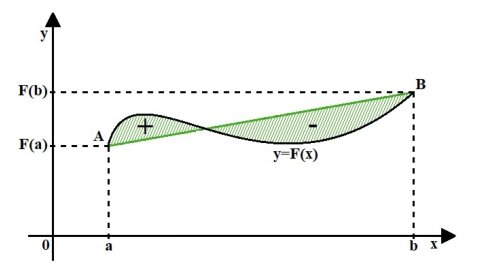
\includegraphics[scale=0.5]{2}}
\caption{Геометричне зображення ітераційний методів:}
{$a$ - сходинки, $b$ - спіраль}
\end{figure}

На площині $xoy$ будуємо графіки функцій $y=x$ та $y=\varphi(x)$. Абсциса точки перетину цих графіків і буде шуканим дійсним коренем $\xi$ рівняння (2). Починаючи з деякої точки $A_0(x_0,\,\varphi(x_0))$, будуємо ламану $A_0B_1A_1B_2A_2\ldots$, ланки якої по черзі паралельні осям $ox$ та $oy$. На кривій $y=\varphi(x)$ розташовані вершини $A_0,\,A_1,\,A_2\ldots$, а вершини $B_1,\,B_2\ldots$ - на прямій $y=x$. Спільні абсциси точок $A_1$ і 
$B_1$, $A_2$ і $B_2$ є послідовними наближеннями $x_1$, $x_2$ кореня $\xi$.

У випадку $a$, коли $0<\varphi'(x)<1$, всі наближення знаходяться з того боку кореня $\xi$, з якого взято нульове наближення $x_0$. Послідовність наближень монотонно прямує до кореня $\xi$, тобто кожне наступне наближення ближче до точного кореня, ніж попереднє.

У випадку $b$, коли $-1<\varphi'(x)<0$, наближення розташовані по черзі то з одного, то з іншого боку від кореня $\xi$. Кожне наступне наближення знаходиться по інший бік від кореня $\xi$, ніж попереднє. У цьому випадку послідовність наближень збігається до кореня $\xi$ за коливним законом. Це означає, що корінь знаходиться завжди між двома сусідніми ітераціями, тому зручно виходити з ітераційного процесу за умови $\left|x_n-x_{n-1}\right|\leqslant\epsilon$. Коли ітераційний процес збігається за коливним законом, то треба прослідкувати, щоб $x_1\in[a,\, b]$.

З рис. 1 видно, що коли в околі кореня $\xi$ функція $\left|\varphi'(x)\right|$ близька до одиниці, то збіжність ітераційного процесу буде дуже повільною, а якщо функція $\left|\varphi'(x)\right|$ близька до нуля, то ітераційний процес збігається дуже швидко.

Якщо $\underset{x\in [a,\, b]}{max}\left|\varphi'(x)\right|>1$, то процес ітерацій може розбігатися. Геометрично це показано на рис. 2 при $\varphi'(x)>1$.

\begin{figure}[h]
\center{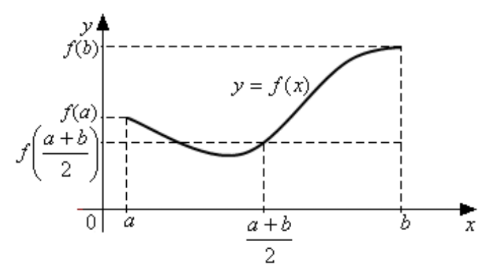
\includegraphics[scale=0.5]{3}}
\caption{Геометричне зображення розбіжного методу}
\end{figure}

Якщо $\varphi'(x)$ не зберігає знак в околі кореня $\xi$, але умова збіжності $\varphi'(x)<1$ виконується, то ітераційний процес буде збігатися за схемою, яка буде якоюсь комбінацією розглянутих двох випадків, показаних на рис. 1. При цьому, для алгоритму не можна дати такого наочного геометричного зображення, як у розглянутих двох випадках.

Ітераційні методи відрізняються один від одного вибором функції $\psi(x)$ у формулі (3).

{\centering \subsection{Метод простої ітерації}}

Цей метод добудемо як частковий випадок ітераційних методів, якщо функцію $\psi(x)$, що знаходиться у правій частині рівності (3), виберемо у вигляді
$$
\psi(x)=-k=const\neq0.
$$

Ітераційна формула (4) для методу простої ітерації приймає вигляд
$$
x_{n+1}=x_n-k\cdot f(x_n),\ n=0,\,1,\ldots
$$

Вважаємо, що на $[a,\, b]$ похідна $f'(x)$ існує, неперервна та зберігає знак (це умова застосування методу). Коефіцієнт $k$ виберемо так, щоб виконувалась умова $\left|\varphi'(x)\right|=\left|1-k\cdot f'(x)\right|<1$ (щоб метод збігався). Останню нерівність можна переписати у вигляді $-1<1-k\cdot f'(x)<1$, або у вигляді системи двох нерівностей
\begin{equation}
\left\{\begin{aligned}
k\cdot f'(x)&>&0,\\
k\cdot f'(x)&<&2
\end{aligned}
\right.
\end{equation}

Нехай $m_1\leqslant\left|f'(x)\right|\leqslant M_1,\ \forall x\in[a,\, b]$. Розглянемо 2 випадки.

1) $f'(x)>0,\ \forall x\in[a,\, b]$. З умов (12) добуваємо нерівності $0<k<\dfrac{2}{f'(x)}$. Звідси випливає, що коефіцієнтом $k$ може бути будь-яке число з проміжку $\left(0;\dfrac{2}{M_1}\right)$.

2) $f'(x)<0,\ \forall x\in[a,\, b]$. З умов (12) добуваємо нерівності $\dfrac{-2}{\left|f'(x)\right|}<k<0$. Звідси випливає, що якщо $k$ належить проміжку $\left(\dfrac{-2}{M_1};0\right)$, то $\left|\varphi'(x)\right|\leqslant q<1$.

В обох випадках швидкість збіжності залежить від числа $q$. Метод буде збігатися найшвидше, якщо 
\begin{equation}
k=\frac{2}{M_1+m_1}\text{ у випадку }f'(x)>0,\ \forall x\in[a,\, b].
\end{equation}
\begin{equation}
k=\frac{-2}{M_1+m_1}\text{ у випадку }f'(x)<0,\ \forall x\in[a,\, b].
\end{equation}

Доведемо формулу (13). Пам'ятаємо, що $q=\underset{x\in [a,\, b]}{max}\left|\varphi'(x)\right|$. Позначимо $\left|\varphi'(x)\right|=\left|1-k\cdot f'(x)\right|\equiv\rho(k,\,x)$. Тут $k$ є аргументом, $x$ - параметром функції $\rho(k,\,x)$. Кожному значенню $x\in[a,\, b]$ відповідає свій графік функції $\rho(k,\,x)$ (рис. 3). Тоді $q=\underset{x\in [a,\, b]}{max}\rho(k,\,x)\equiv q(k)$. Оскільки $f'(x)>0$, $\forall x\in[a,\, b]$, то $k\in\left(0;\dfrac{2}{M_1}\right)$. Позначимо $k_{\text{опт}}$ таке значення аргументу $k$, при якому  
$q(k_{\text{опт}})$ буде мінімальним, тобто
$$
q(k_{\text{опт}})=\underset{k\in\left(0;\frac{2}{M_1}\right)}{min}q(k).
$$

Задачу мінімізації функції $q(k)$ розв'язуємо графічно. З рис. 3 видно, що функція $q(k)$ своє мінімальне значення приймає в точці $D$, де
$$
1-m_1\cdot k_{\text{опт}}=-(1-M_1\cdot k_{\text{опт}}).
$$

Звідси знаходимо $(M_1+m_1)\cdot k_{\text{опт}}=2$, тобто $k_{\text{опт}}=\dfrac{2}{M_1+m_1}$. Отже, формула (13) доведена.

Для випадку $f'(x)<0,\ \forall x\in[a,\, b]$ формула (14) доводиться аналогічно.

Зауважимо, що $\varphi'(\xi)=1-k\cdot f'(\xi)\neq0$. Це означає, що порядок збіжності методу простої ітерації дорівнює одиниці.
\begin{figure}[h]
\center{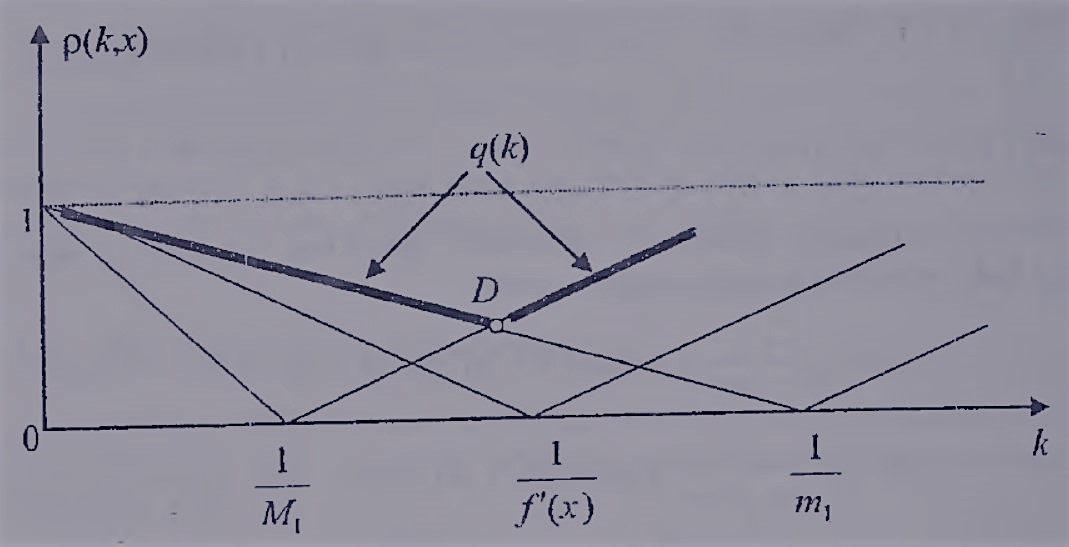
\includegraphics[scale=0.5]{4}}
\caption{Графічне доведення формули (13)}
\end{figure}

{\centering \subsection{Метод Ньютона}}

Цей метод одержимо, якщо функцію $\psi(x)$, шо стоїть у правій частині формули (3), виберемо у вигляді $\psi(x)=-\dfrac{1}{f'(x)}$, тоді $\varphi(x)=x-\dfrac{f(x)}{f`(x)}$. Вважаємо, що на $[a,\, b]$ похідні $f'(x),\ f''(x)$ існують, неперервні та зберігають знак (це умови застосування методу дотичних). Знаходимо похідну $\varphi'(x)$
\begin{equation}
\varphi'(x)=1-\frac{f'(x)}{f'(x)}+\frac{f(x)f''(x)}{(f'(x))^2}=\frac{f(x)f''(x)}{(f'(x))^2}.
\end{equation}

Як видно з (15), $\varphi(\xi)=0$. Це означає, що існує такий окіл точки $\xi$, де $\underset{x\in[a,\, b]}{max}\left|\varphi'(x)\right|<1$, тобто ітераційний процес буде збігатися. Отже, якщо метод Ньютона розбігається, то треба звузити відрізок $[a,\, b]$. З (15) знаходимо $\varphi''(\xi) = \dfrac{f''(\xi)}{f'(\xi)}\neq0$. Це означає, що в умовах (11) $m = 2$, тобто порядок збіжності методу Ньютона дорівнює двом.

Запишемо ітераційну формулу методу Ньютона
\begin{equation}
x_{n+1}=x_n-\frac{f(x_n)}{f'(x_n)},\ n=0,\,1,\ldots
\end{equation}

Якщо $x_0$ вибрати так, щоб $f(x_0)\cdot f''(x_0) > 0$, то $\varphi'(x_0) > 0$, тому всі наближення, починаючи з $x_0$, будуть знаходитись з одного і того ж боку від кореня $\xi$ (з того, де розташоване $x_0$) та будуть прямувати до $\xi$ монотонно.

Якщо $x_0$ вибрати так, щоб $f(x_0)\cdot f''(x_0) < 0$, то наближення $x_1$ буде з іншого боку від кореня $\xi$, ніж $x_0$, і якщо $x_1$ не вийде за межі відрізка $[a,\, b]$, то всі наступні наближення $x_2,\,x_3,\ldots$ будуть з того боку від кореня $\xi$, з якого знаходиться $x_1$. Отже, послідовність $x_1,\,x_2,\,x_3,\ldots$ буде монотонно прямувати до кореня $\xi$. Якщо $x_1$ вийде за межі $[a,\,b]$, то треба змінити $x_0$.

Метод Ньютона має своє власне геометричне зображення, показане на рис. 4. Ітераційну формулу (16) можна добути з геометричного зображення методу, для цього треба записати рівняння дотичної до графіка функції $y = f(x)$ в точці $(x_n, f(x_n))$
$$
y = f(x_n) + (x - x_n)f'(x_n).
$$

Точка перетину цієї дотичної з віссю абсцис має координати $(x_{n+1}, 0)$. Підставивши координати цієї точки в рівняння дотичної, добудемо формулу (16).
\begin{figure}[h]
\center{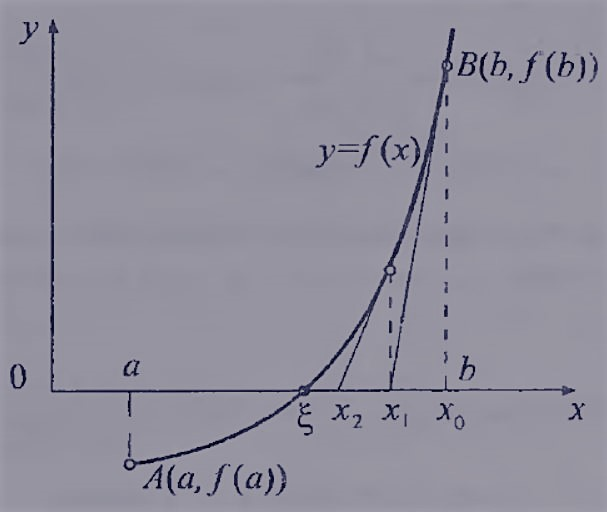
\includegraphics[scale=0.5]{5}}
\caption{Графічне зображення методу Ньютона}
\end{figure}

{\centering \subsection{Метод хорд}}

Цей частковий випадок ітераційних методів добудемо, якщо функцію $\psi(x)$, шо стоїть у правій частині формули (3), виберемо у вигляді 
$$
\psi(x) = - \frac{x - c}{f(x) - f(c)},
$$
де $c$ - якась точка з $[a,\,b]$. З формули (3) маємо
$$
\varphi = x - \frac{(x - c)f(x)}{f(x) - f(c)}.
$$

Ітераційна формула методу хорд має вигляд
\begin{equation}
x_{n+1} = x_n - \frac{(x_n - c)f(x_n)}{f(x_n) - f(c)},\ n = 0,\,1,\,2,\ldots
\end{equation}
Щоб проаналізувати особливості збіжності методу, знайдемо похідну $\varphi'(x)$.
$$
\varphi'(x) = 1 - \left(\frac{x - c}{f(x) - f(c)}\right)'_x \cdot f(x) - \frac{(x - c) \cdot f'(x)}{f(x) - f(c)} =$$$$
= 1 - f(x)\left(\frac{1}{f(x) - f(c)} - \frac{(x - c) \cdot f'(x)}{(f(x) - f(c))^2}\right) - \frac{(x - c)\cdot f'(x)}{f(x) - f(c)} = $$$$
= 1 - \frac{f(x)}{f(x) - f(c)} + \frac{(x - c)f'(x)}{f(x) - f(c)}\left( \frac{f(x)}{f(x) - f(c)} - 1 \right) = $$$$
= \frac{f(c)}{(f(x) - f(c))^2}(f(c)-f(x)+(x-c)f'(x)).$$
Якщо скористатися наступним розвиненням
$$
f(c) = f(x) + (c - x)\cdot f'(x) + \frac{(c - x)^2}{2!}f''(\widetilde{ x}),\  \widetilde{x}\in (x,\,c),
$$
то шукану похідну $\varphi'(x)$ можна переписати у вигляді
\begin{equation}
\varphi'(x) = \frac{f(c)\cdot f''(\widetilde{x}) \cdot (c - x)^2}{2(f(x) - f(c))^2},\ \widetilde{x}\in (x,\,c).
\end{equation}

Похідні $f'(x),\ f''(x)$ зберігають знак на $[a,\,b]$ (це умова застосування методу хорд), тому якщо точку $c$ вибрати так, щоб виконувалася нерівність
\begin{equation}
f(c)\cdot f''(c) > 0,
\end{equation}
то на всьому відрізку $[a,\,b]$ буде виконуватись умова $\varphi'(x) > 0$, а це означає, що послідовність наближень $\left\lbrace x_n \right\rbrace_{n = 0}^\infty$ буде прямувати до кореня $\xi$ монотонно. Якщо при цьому нульове наближення $x_0$ вибрати так, щоб
\begin{equation}
f(x_0)\cdot f(c) < 0,
\end{equation}
то в знаменнику ітераційної формули (17) модулі чисел $f(x_n)$ та $f(c)$ будуть додаватися.

Коли число $c$ взято достатньо близьким до точного кореня $\xi$, то, як видно з (18), $\varphi'(x)$ буде малим за модулем числом за рахунок множника $f(c)$ і тому існує такий окіл точки $\xi$, в якому буде виконуватися нерівність $\left|\varphi'(x)\right| < 1$, а це означає, що ітераційний процес буде збігатися до точного кореня $\xi$.

З формули (18) маємо $\varphi'(\xi) = \dfrac{f(c)\cdot f''(\tilde{x})\cdot (c - \xi)^2}{2(f(c))^2} \neq 0$. Це означає, що в умовах (11) $m = 1$, тобто метод хорд має перший порядок збіжності.

Метод хорд має своє власне геометричне зображення, показане на рис. 5.

Ітераційну формулу (17) можна добути з геометричного зображення методу хорд. Для цього запишемо рівняння прямої, що проходить через дві точки з координатами $(x_n,\,f(x_n))$ та $(c,\,f(c))$
$$
\frac{x - x_n}{c - x_n} = \frac{y - f(x_n)}{f(c) - f(x_n)}.
$$

\begin{figure}[h]
\center{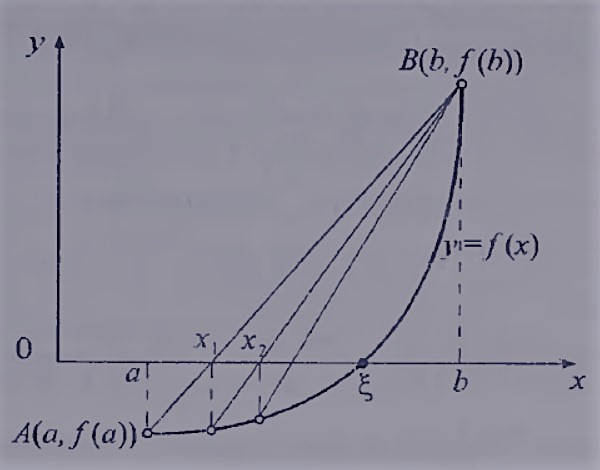
\includegraphics[scale=0.5]{6}}
\caption{Графічне зображення методу хорд}
\end{figure}

Ця пряма (хорда) перетинає вісь абсцис у точці з координатами $(x_{n+1},\,0)$. Підставивши координати цієї точки до рівняння хорди, добудемо формулу (17).

{\centering \subsection{Комбінований метод}}

Методи хорд і дотичних дають наближення кореня з різних боків. Тому часто їх застосовують у комбінації один з одним, і уточнення кореня відбувається швидше.

З урахуванням типу графіка функції ці методи комбінують так. 

Якщо $f'(x_0)f''(x_0) > 0$, то метод хорд дає наближене значення кореня з недостачею, а метод дотичних - з надлишком.

Якщо ж $f'(x_0)f''(x_0) < 0$, то за методом хорд отримаємо значення кореня $\alpha$ з надлишком, а методом дотичних - з недостачею.

У всіх випадках справжній корінь розміщений між наближеними значеннями, отриманими за методами хорд і дотичних, тобто
$$
a < \underline{x_n} < \alpha < \overline{x_n} < b,
$$
де $\underline{x_n}$ - наближене значення кореня з недостачею; $\overline{x_n}$ - наближене значення кореня з надлишком.

\begin{itemize}
\item Нехай $f'(x_0)f''(x_0) > 0$, тоді з кінця $a$ лежать наближені значення, отримані за методом хорд, а з кінця $b$ - за методом дотичних. Ітераційний процес матиме вигляд
$$
\underline{x_0} = a;\ \overline{x_0} = b;
$$
$$
\underline{x_n} = \underline{x_{n-1}} - \frac{f(\underline{x_{n-1}})(\overline{x_{n-1}} - \underline{x_{n-1}})}{f(\overline{x_{n-1}}) - f(\underline{x_{n-1}})}; \eqno(1)
$$
$$
\overline{x_n} = \overline{x_{n-1}} - \frac{f(\overline{x_{n-1}})}{f'(\overline{x_{n-1}})};\ n = 1,\,2,\ldots
$$
\item Нехай $f'(x_0)f''(x_0) < 0$, тоді, навпаки, з кінця $a$ є наближені значення кореня за методом дотичних, а з кінця $b$ - за методом хорд
$$
\underline{x_0} = a;\ \overline{x_0} = b;
$$
$$
\underline{x_n} = \underline{x_{n-1}} - \frac{f(\underline{x_{n-1}})}{f'(\underline{x_{n-1}})}; \eqno(2)
$$
$$
\overline{x_n} = \overline{x_{n-1}} - \frac{f(\overline{x_{n-1}})(\overline{x_{n-1}} - \underline{x_{n-1}})}{f(\overline{x_{n-1}}) - f(\underline{x_{n-1}})};\ n = 1,\,2,\ldots
$$
\end{itemize}

Ітераційний процес закінчується, коли $\left| \overline{x_n} - \underline{x_n} \right| < \epsilon$. За значення кореня обираємо середину звуженого проміжку
$$
a = \frac{1}{2}(\overline{x_n} + \underline{x_n}).
$$

Комбінований метод є нестаціонарним методом уточнення дійсних коренів рівняння $f(x) = 0$. Збігається він значно швидше, ніж метод дотичних.

Метод хорд є ітераційним методом першого порядку, а метод Ньютона - другого порядку. Метод Ньютона можна застосовувати і для знаходження комплексних коренів. Тоді для випадку дійсної функції $f(x)$ початкове наближення $х_0$ повинно бути комплексним числом. 

\textbf{Зауваження 1.} За умов теореми метод ітерацій збігається для довільного початкового значення $x_0 \in [a,\,b]$. Завдяки цьому він є самовиправним, тобто окрема помилка в обчисленнях не впливає на кінцевий результат, бо помилкове значення можна розглядати як нове початкове наближення $x_0$. Ця властивість робить метод ітерацій найнадійнішим методом обчислень.

На практиці часто виникає ситуація, коли проміжок $[a,\,b]$ досить великий і умова $|\varphi'(x)| < 1$ виконується лише в деякому околі кореня, тому в разі невдалого вибору початкового наближення $x_0$ послідовні наближення $x_n = \varphi(x_{n-1})(n = 1,\,2,\ldots)$ можуть вийти за межі проміжку $[a,\,b]$.

\textbf{Зауваження 2.} У методі дотичних бачимо, що чим більше числове значення похідної $f'(x)$ в околі заданого кореня, тим менша поправка, яку требя додати до $n$-го наближення, щоб отримати $(n+1)$-ше наближення. Тому метод Ньютона особливо зручно застосовувати тоді, коли в околі заданого кореня графік функції має велику стрімкість. Однак коли числове значення похідної $f'(x)$ біля кореня мале, то поправки будуть великими й обчислення кореня за цим методом може виявитись довгим, а іноді й зовсім неможливим. Отже, якщо крива $y = f(x)$ поблизу точки перетину з віссю $Ox$ майже горизонтальна, то застосовувати метод Ньютона для розв'язування рівняння $f(x) = 0$ не рекомендуємо.
\newpage
{\centering \section{Чисельний експеримент та аналіз результатів}}
{\centering \subsection{Опис програмної реалізації}}

\end{document} 